\documentclass[12pt,letterpaper]{article}

% PAM development roadmap; portable pdfLaTeX source.
\usepackage[T1]{fontenc}
\usepackage[utf8]{inputenc}
\usepackage{newtxtext,newtxmath} % Times-style text and mathematics
\usepackage[margin=1in,headheight=15pt]{geometry}
\usepackage{microtype}
\usepackage{amsmath}
\usepackage{enumitem}
\usepackage{array,booktabs,tabularx,longtable}
\usepackage{tikz}
\usetikzlibrary{arrows.meta,positioning,shapes.geometric}
\usepackage{listings}
\usepackage{xcolor}
\usepackage{fancyhdr}
\usepackage{titlesec}
\usepackage{hyperref}
\usepackage{xurl}
\usepackage{caption}
\hypersetup{colorlinks=true,linkcolor=blue!45!black,urlcolor=blue!45!black,pdftitle={PAM 1.0: The Road to Blender},pdfauthor={PAM development roadmap}}

\definecolor{pamblue}{HTML}{426B88}
\definecolor{pamteal}{HTML}{277D75}
\definecolor{pampurple}{HTML}{775BA0}
\definecolor{codebg}{HTML}{F5F7F8}
\definecolor{coderule}{HTML}{DDE3E6}
\definecolor{codeword}{HTML}{1E4663}
\titleformat{\section}{\normalfont\Large\bfseries\color{pamblue}}{\thesection}{0.8em}{}
\titleformat{\subsection}{\normalfont\large\bfseries}{\thesubsection}{0.7em}{}
\setlist[itemize]{topsep=4pt,itemsep=2pt,parsep=0pt,leftmargin=*}
\setlist[enumerate]{topsep=4pt,itemsep=3pt,parsep=0pt,leftmargin=*}
\renewcommand{\arraystretch}{1.16}
\captionsetup{font=small,labelfont=bf}
\lstdefinestyle{pamjson}{
 basicstyle=\ttfamily\footnotesize,
 backgroundcolor=\color{codebg},
 frame=single,rulecolor=\color{coderule},
 breaklines=true,breakatwhitespace=false,
 showstringspaces=false,
 columns=fullflexible,
 keepspaces=true,
 tabsize=2,
 keywordstyle=\color{codeword},
 literate={\_}{{\_}}1,
 xleftmargin=0.8em,xrightmargin=0.8em,
 aboveskip=8pt,belowskip=8pt
}
\lstset{style=pamjson}
\pagestyle{fancy}
\fancyhf{}
\fancyhead[L]{\small PAM 1.0: The Road to Blender}
\fancyhead[R]{\small Development outline}
\fancyfoot[C]{\thepage}
\setlength{\headsep}{19pt}
\newcommand{\file}[1]{\texttt{\detokenize{#1}}}
\newcommand{\priority}[1]{\noindent\textbf{Priority:} #1\par\smallskip}
\newcommand{\completion}[1]{\par\medskip\noindent\textbf{Completion test.} #1\par}
\newcommand{\pam}{\textsc{pam}}

\begin{document}
\begin{center}
{\huge\bfseries PAM 1.0: The Road to Blender}\par
\vspace{0.5em}
{\Large Programming Roadmap for Choreography and Stateful Props}\par
\vspace{0.7em}
{\normalsize Development outline --- November 18, 2026}\par
\vspace{0.3em}
{\small Repository: \url{https://github.com/wdjoyner/pam}}\par
\end{center}
\vspace{0.5em}

\begin{abstract}
The objective is to extend Pose And Motion (PAM) into a screenplay-driven animation engine capable of producing a \emph{complete, carefully timed Manim performance} that can later be rendered in Blender without changing the choreography. The plan consists of nine incremental milestones, with \emph{Abraham and Isaac, Revisited} (Draft 2) as the principal integration test. Its emphasis is on dependable choreography, interaction constraints, composite prop state, reproducible timing, and trace fidelity---before Blender cosmetics.
\end{abstract}

\tableofcontents
\clearpage

\section{Architectural objective}

The central design decision is to maintain \textbf{one executable performance specification}, rather than two separately authored animations. The basic flow is
\[
\text{Fountain+}\longrightarrow\text{PAM JSON}\longrightarrow
\text{Manim runtime}\longrightarrow\text{semantic motion trace}
\longrightarrow\text{Blender}.
\]
The Manim runtime determines character movement, interactions, timing, camera shots, and prop behavior. Blender replaces or enhances visual representations while retaining those decisions. A corrected gesture or comic pause should require editing the performance only once, after which both outputs can be regenerated.

\begin{figure}[htbp]
\centering
\begin{tikzpicture}[
 node distance=0.35cm,
 box/.style={draw=none,rounded corners=3pt,align=center,text=white,
   text width=11cm,minimum height=1.05cm,inner sep=5pt,font=\small},
 arrow/.style={-{Stealth[length=3mm]},semithick,draw=black!65}]
\node[box,fill=pamblue] (f) {\textbf{Fountain+ screenplay}\\Dialogue, scenes, camera instructions, production cues};
\node[box,fill=pamblue,below=of f] (j) {\textbf{PAM JSON + cast and prop registries}\\Authoritative executable performance};
\node[box,fill=pamteal,below=of j] (r) {\textbf{PAM animation runtime}\\Choreography, constraints, prop states, timing};
\node[box,fill=pamteal,below=of r] (m) {\textbf{Manim animatic}\\Complete performance and editorial reference};
\node[box,fill=pampurple,below=of m] (t) {\textbf{PAM motion + semantic-event trace}\\Joint motion, camera, prop states, synchronized timebase};
\node[box,fill=pampurple,below=of t] (b) {\textbf{Blender renderer}\\Geometry and visual refinement without re-choreography};
\draw[arrow] (f)--(j); \draw[arrow] (j)--(r); \draw[arrow] (r)--(m);
\draw[arrow] (m)--(t); \draw[arrow] (t)--(b);
\end{tikzpicture}
\caption{The Manim animation is the reference performance. Blender consumes its recorded motion and semantic events rather than interpreting the screenplay independently.}
\label{fig:architecture}
\end{figure}

A practical implementation principle follows: build \emph{constraints}, \emph{choreography}, and \emph{prop state} as three distinct subsystems, coordinated by a single timeline. The existing PAM runtime and its instrumentation hooks should be extended incrementally, not replaced.

\section{Milestone 1: Establish a regression-tested baseline}
\priority{Critical}

\noindent\textbf{Modules:} \file{pam_player.py}, \file{pam_trace.py}, \file{trace2blender.py}, and a new \file{tests/} directory.

Before changing functionality, protect existing PAM behavior. The current code already includes character scaling, locomotion, prop attachments, camera controls, trace generation, instrumentation through \file{pam/hooks.py}, and warning output such as \file{PAM_WARNINGS_JSON}.

\subsection{Programming tasks}
\begin{enumerate}
\item Record the current Git commit and reference version for reproducibility.
\item Add a \file{pytest} test suite and identify existing PAM examples suitable as regression fixtures.
\item Test character scaling, locomotion, named poses, prop attachment and handoff, camera movement, and motion-trace generation.
\item Add a JSON validator that rejects unknown actions, invalid joint names, negative durations, and references to missing characters or props.
\item Capture and report warnings from \file{fountain2pam.py} rather than silently ignoring unresolved \file{# REVIEW} comments.
\item Provide a command for validating an animation without rendering a video.
\end{enumerate}

This stage should involve little or no restructuring of the runtime.
\completion{Existing PAM scripts continue to execute, and their basic motion, camera, and prop behavior remain unchanged.}

\section{Milestone 2: Define a synchronized animation timeline}
\priority{Critical}

\noindent\textbf{New module:} \file{pam/timeline.py}.\\
\textbf{Modify:} \file{pam/actions.py}, \file{pam_player.py}, \file{pam/hooks.py}.

PAM already supports action durations, \file{Scene.play}, \file{Scene.wait}, and camera timing. A complete comic performance needs an explicit mechanism for synchronizing parallel actions, dialogue, camera cuts, and intentional pauses.

The proposed timeline should use an internal integer frame clock, initially at 30 frames per second; legacy actions specified in seconds would be converted at the timeline boundary. This avoids accumulating floating-point timing drift and allows an editor to specify exact frame counts for physical gags.

\subsection{Proposed action format}
The following is an \emph{interface proposal}, not existing PAM syntax:
\begin{lstlisting}
{
  "action": "sequence",
  "id": "s02_pull_attempt",
  "fps": 30,
  "steps": [
    {
      "action": "grip_character",
      "who": "abraham",
      "target": "isaac",
      "duration_frames": 12
    },
    {
      "action": "paired_action",
      "name": "pull_immovable",
      "a": "abraham",
      "b": "isaac",
      "duration_frames": 36
    },
    {
      "action": "slip_on_back",
      "who": "abraham",
      "duration_frames": 9
    },
    {
      "action": "hold",
      "duration_frames": 18
    }
  ]
}
\end{lstlisting}

\subsection{Runtime responsibilities}
\begin{itemize}
\item Sequential and simultaneous actions, with deterministic ordering.
\item Fixed-duration gestures and pauses (including explicit \emph{holds}).
\item Exact onset and completion times for contact constraints.
\item Camera cuts on specified frames.
\item Synchronization of sound effects and dialogue with movement.
\item Named performance beats that can be revised without rewriting a scene.
\end{itemize}

Stillness is a deliberate acting choice, not merely an absence of animation. The timeline must represent it explicitly.
\completion{Two actors perform overlapping movements while the camera cuts and dialogue begins at exact designated frames. Repeated renders have identical timing.}

\section{Milestone 3: Reusable choreography and interaction constraints}
\priority{Critical---the principal new engine feature}

\noindent\textbf{New modules:} \file{pam/choreography.py}, \file{pam/constraints.py}.\\
\textbf{Modify:} \file{pam/paired_poses.py}, \file{pam/poses.py}, \file{pam/figure.py}, \file{pam/actions.py}.

PAM already supports individual poses and gestures, but interacting characters frequently require painstaking manual coordination. Its existing \file{paired_poses.py} is primarily an authoring convenience: it emits standard actions and does not provide a general constraint engine for moving actors in contact.

\subsection{Initial constraint types}
\begin{table}[htbp]
\centering
\begin{tabularx}{\textwidth}{@{}>{\ttfamily}l X@{}}
\toprule
\normalfont\textbf{Constraint} & \textbf{Purpose}\\
\midrule
joint\_to\_joint & Keep Abraham's hand attached to Isaac's wrist.\\
joint\_to\_prop & Keep Isaac's hand on the knife or phone.\\
root\_lock & Keep Isaac stationary while Abraham pulls.\\
joint\_to\_point & Keep a hand, foot, or prop at a fixed spatial target.\\
\bottomrule
\end{tabularx}
\caption{The first four contact constraints. Each has an explicit active interval.}
\end{table}

In the \file{pull_immovable} action, Isaac's root remains locked and Abraham's hand remains attached to Isaac's wrist while Abraham leans backward. When Abraham slips, the wrist constraint is released and a fast fall action begins. The important abstraction is the temporary relation between character skeletons, not a collection of hard-coded screen coordinates.

\subsection{First choreography routines}
\begin{longtable}{@{}>{\ttfamily\small}p{0.31\textwidth}p{0.09\textwidth}p{0.52\textwidth}@{}}
\toprule
\normalfont\textbf{Routine} & \textbf{Scene} & \textbf{Narrative function}\\
\midrule
\endfirsthead
\toprule
\normalfont\textbf{Routine} & \textbf{Scene} & \textbf{Narrative function}\\
\midrule
\endhead
pull\_immovable & 2 & Abraham strains while Isaac remains still.\\
slip\_on\_back & 2 & Sudden loss of balance.\\
cork\_pop\_up & 2 & Isaac pulls Abraham upright effortlessly.\\
mismatched\_hug & 2 & Abraham cannot reach around Isaac.\\
catch\_by\_collar & 3 & Isaac catches his falling father.\\
tie\_wrist\_loop & 4 & Abraham struggles with the rope.\\
reach\_and\_tighten & 5 & Isaac accidentally tightens his knot.\\
altar\_tumble\_hug & 6 & Both characters tumble while embracing.\\
\bottomrule
\end{longtable}

Begin with deterministic key poses and simple constraint correction. A complete inverse-kinematics solver might be valuable later, but it is not initially necessary: existing graph skeletons allow geometric adjustment of elbows, shoulders, hips, and knees between specified poses.

\subsection{Scale-aware choreography}
Constraints must operate on \emph{resolved, scaled joint positions}. For instance, \file{mismatched_hug} should measure Isaac's actual torso width, while Abraham's reach is determined by his arm lengths. It should not rely on fixed screen coordinates. This preserves the joke if the relative size of the characters changes.

\completion{Change Isaac's scale from 1.15 to 1.30 and replay the Scene 2 physical gags. The movements remain coherent without manual re-blocking.}

\section{Milestone 4: Stateful composite props}
\priority{Critical}

\noindent\textbf{New module:} \file{pam/prop_states.py}.\par
\noindent\textbf{Modify:} \file{pam/props_core.py}, \file{pam/props_carried.py}.\par
\noindent\hspace*{1.2em}\file{pam/props_environment.py}, \file{pam_player.py}, and \file{pam/hooks.py}.

PAM already has a prop scene graph, attachment points, and handoff events. The missing abstraction is a generic method for a prop to change its structure or appearance as part of the performance. Prefer a \emph{state machine} to separate hard-coded actions for every individual object.

\subsection{Composite knife example}
This is a proposed definition, not current PAM syntax:
\begin{lstlisting}
{
  "id": "knife",
  "type": "composite_prop",
  "initial_state": "intact",
  "parts": {
    "handle": {"type": "knife_handle"},
    "blade":  {"type": "knife_blade"}
  },
  "states": {
    "intact": {"connected": true},
    "broken": {"connected": false}
  }
}
\end{lstlisting}

A generic \file{prop_transition} action would indicate which pieces separate, which attachments release, and which animations play. The trace must preserve prop identities and transition events; positions alone do not convey enough information for Blender to reproduce the correct geometry.

\subsection{First four prop families}
\begin{itemize}
\item \textbf{Knife---composite prop.} States \file{intact}, \file{broken}, \file{blade_carried}, and \file{blade_embedded}. The handle and blade retain separate identities after breaking.
\item \textbf{Rope---deformable attachment.} States \file{loose}, \file{tied}, \file{tightened}, and \file{snapped}. The loop follows Isaac's wrists until it breaks; after the snap, two separate pieces recoil.
\item \textbf{Scroll---text-bearing prop.} States \file{rolled}, \file{unrolled}, \file{edited}, and \file{trailing}. Text revisions and geometry transformations are separate dimensions of its state.
\item \textbf{Phone---interactive display.} States \file{standby}, \file{recording}, and \file{live}. The screen display and viewer count can change independently of the phone's spatial location.
\end{itemize}

\subsection{Cross-scene continuity}
After the knife breaks in Scene 2, its handle and blade must remain separate objects. The blade should be located in Abraham's satchel during Scene 4 and embedded in the altar during Scene 5, according to explicit state and attachment data. The runtime must not infer this continuity from whichever items happened to be visible in a prior Manim frame.

The same principle governs the rope's knot and the scroll's revisions. State continuity should be testable without rendering graphics.
\completion{Every knife component reaches its expected state and location, with no disappearing or duplicated pieces. The state tests pass independently of the renderer.}

\section{Milestone 5: Fountain+ compilation and shot direction}
\priority{High}

\noindent\textbf{Modify:} \file{fountain2pam.py}, \file{pam_player.py}.\\
\textbf{Proposed new module:} \file{pam/shot_targets.py}.

The screenplay should remain readable as a screenplay, not become an enormous collection of low-level animation commands. Preserve the existing Fountain+ metadata conventions, and place choreography that cannot be confidently inferred from ordinary prose in a separate animation-cue file.

\subsection{Suggested project layout}
\begin{lstlisting}
projects/abraham_isaac/
    source/
        screenplay.fountain
    cast/
        characters.json
    props/
        prop_definitions.json
    cues/
        animation_cues.json
    scenes/
        scene01.json
        scene02.json
        ...
\end{lstlisting}

The screenplay maintained in the \file{writing-guides/shorts} project can remain the authoritative literary version. The animation project may contain its production source or a reproducible reference to it.

\subsection{Two targeted compiler improvements}
\begin{enumerate}
\item \textbf{Explicit choreography cues.} Continue compiling familiar actions automatically. For complex movements, match a stable screenplay beat identifier to a curated PAM action sequence. This protects hand-authored choreography from being overwritten when Fountain is recompiled.
\item \textbf{Prop-aware camera framing.} Existing camera code can target named characters and props. Improve inserts by calculating framing from an object's bounding box and intended screen margin, rather than relying principally on horizontal position. This is important for the scroll, the broken knife, and the phone.
\end{enumerate}

\completion{Recompiling the Fountain screenplay does not erase hand-authored choreography or incorrectly frame the critical inserts.}

\section{Milestone 6: The complete Manim performance}
\priority{High---the first major artistic deliverable}

This milestone is deliberately independent of Blender. All six scenes must become a complete enough animated performance that a viewer can assess the comedy without needing to read the screenplay. The Manim render should include dialogue, speech bubbles or voices, physical acting, prop effects, camera work, intentional holds, and transitions.

\subsection{Scene-by-scene acceptance tests}
\begin{longtable}{@{}p{0.24\textwidth}p{0.69\textwidth}@{}}
\toprule
\textbf{Scene} & \textbf{Required outcome}\\
\midrule
\endfirsthead
\toprule
\textbf{Scene} & \textbf{Required outcome}\\
\midrule
\endhead
1---The Manuscript & Abraham writes; the scroll insert is readable; the question-mark gag lands.\\
2---The Invincible & Scale contrast, wrist pull, fall, cork-pop, broken knife, and hug all read clearly.\\
3---The Climb & Isaac's effortless movement contrasts with Abraham's struggles.\\
4---The Altar & Props are staged correctly; rope and phone interactions are clear.\\
5---Live & The accidental livestream, blade incident, and dramatic silence work.\\
6---The Revision & Rope snap, embrace, tumble, scroll editing, and final image are complete.\\
\bottomrule
\end{longtable}

\subsection{Performance profiles and acting}
Create optional \emph{performance profiles} for recurring behaviors. Abraham's profile could contain hesitant speech preparation, finger-counting, anxiety, exaggerated effort, and sudden decisiveness. Isaac's could include relaxed posture, casual strength, cheerful reactions, and fast recovery.

Avoid mechanically attaching the same gesture to every dialogue line. Where appropriate, an action should have four phases:
\[
\text{anticipation}\;\longrightarrow\;
\text{action}\;\longrightarrow\;
\text{reaction}\;\longrightarrow\;
\text{recovery}.
\]
For the cork-pop gag, Isaac offers his hand, Abraham accepts, the abrupt movement occurs, and the image holds briefly before Abraham speaks. Each phase's duration should be adjustable without rewriting the choreography.

The most important dramatic choice in Scene 5 is to permit stillness after the knife incident: the performance turns from staged slapstick toward a sincere exchange between father and son.

\completion{The complete six-scene Manim video is independently watchable. Its physical jokes and emotional turn are comprehensible without the script. This is a valid production milestone even before Blender is used.}

\section{Milestone 7: Extend the semantic motion trace}
\priority{High}

\noindent\textbf{Modify:} \file{pam/hooks.py}, \file{pam_trace.py}.

The existing PAM trace already records skeletal motion, actions, camera transforms, overlays, prop positions, attachments, and visibility. Extend this format rather than replacing it. The main addition is a stream of typed semantic events aligned with the same integer frame clock.

\subsection{Example event}
\begin{lstlisting}
{
  "frame": 412,
  "event": "prop_state_changed",
  "prop": "knife",
  "from": "intact",
  "to": "broken"
}
\end{lstlisting}

Also record the active intervals of contact constraints, creation of new prop components, and updates to text displayed on surfaces.

\subsection{Resolved motion versus recomputed constraints}
Store \emph{resolved movement}, not merely the constraints that produced it. Manim calculates actual joint positions after constraint correction. The tracer stores those positions and the semantic events Blender needs to select or instantiate the right geometry. Blender should \emph{not} solve the choreography a second time.

\completion{A trace replay reconstructs the Manim performance's joint movement, camera cuts, prop states, and frame timings within specified numerical tolerances.}

\section{Milestone 8: Blender parity before embellishment}
\priority{After completion of the Manim performance}

\noindent\textbf{Modify:} \file{trace2blender.py}.

The first Blender target is not more attractive rendering but \emph{correct reproduction}. Begin with plain capsule figures, simple meshes, and basic lighting. Check paired actions, separated knife pieces, rope attachments, text changes, and camera motions against Manim.

After parity is demonstrated, improve the character meshes, robes, sandals, rocks, desert environments, lighting, and scroll-ribbon deformation. Keep these appearance changes in asset and material layers with minimal effect on choreography code.

\completion{Blender matches the Manim animation in movement, staging, prop identity, and timing before detailed geometry and materials are added.}

\section{Milestone 9: Documentation and release readiness}
\priority{Release readiness}

Document generic PAM features in the main repository:
\begin{itemize}
\item Timeline and sequence formats, including parallel actions and holds.
\item Choreography routines and scale-aware interaction constraints.
\item Composite-prop definitions, states, transitions, and continuity.
\item Fountain+ cue integration and prop-aware camera framing.
\item Semantic trace events and Blender reconstruction guarantees.
\item Small, self-contained, automated examples and regression tests.
\end{itemize}

The six-scene Abraham--Isaac animation becomes a substantial integration example demonstrating the end-to-end system. Reserve the \emph{PAM 1.0} label for a release in which the regression tests and Manim performance acceptance criteria pass.

\section{Implementation dependencies and sequencing}

\begin{enumerate}
\item Regression tests and validation.
\item Timeline and synchronized actions.
\item Contact constraints and choreography primitives.
\item Stateful composite props.
\item Fountain+ integration and prop camera targets.
\item Complete Manim short.
\item Semantic trace export.
\item Blender motion parity.
\item Documentation and release tests.
\end{enumerate}

The first four stages involve the most significant engine-development work. The later stages primarily integrate, validate, and package those generic capabilities. In particular, postpone detailed Blender cosmetics until choreography and state transitions can be verified in Manim.

\section{Recommended first coding task: a vertical slice}

Start with one \emph{complete choreography example}, not nine disconnected implementation branches. The Scene 2 failed wrist-pull is the best initial vertical slice.

It requires:
\begin{enumerate}
\item A timeline with discrete durations and an explicit pause.
\item Two differently scaled characters, Abraham and Isaac.
\item One wrist-to-wrist contact constraint.
\item A root lock that makes Isaac immovable.
\item Constraint release at a specified frame.
\item Abraham's sudden fall followed by a comic hold.
\item Consistent replay and a regression test.
\end{enumerate}

Once this works, add the breakaway knife as the first prop-state test. Together these two short sequences exercise almost every important new concept while keeping debugging manageable.

The primary architectural recommendation is to make \textbf{constraints, choreography, and prop states three separate subsystems joined by a single timeline}. This allows additional physical gags without continually rewriting \file{pam_player.py} and gives PAM a reusable base for later projects, including the rest of \emph{Abraham and Isaac, Revisited}.

\section*{Concluding principle}
\addcontentsline{toc}{section}{Concluding principle}

\begin{quote}
\emph{Build a better choreography and prop-state system before spending effort on Blender cosmetics. Treat the Manim animatic as the complete reference performance, not a disposable rough visualization.}
\end{quote}

This is the foundation to establish before extending the Blender renderer.

\end{document}
